\newpage
\section{Présentation de l'entreprise}

L'HESTIM Engineering School (Hautes Études des Sciences et Techniques de
l'ingénierie et du Management) est un établissement privé d'enseignement
supérieur basé à Casablanca, au Maroc. Fondée en 2006, elle forme chaque
année plusieurs centaines d'étudiants dans les domaines de l'ingénierie et
du management. HESTIM fonctionne comme une entreprise de formation et de
services académiques, structurée pour répondre aux besoins croissants des
secteurs industriels et technologiques au Maroc et à l'international.

\begin{figure}[H]
	\centering
	
\includegraphics[width=0.35\textwidth]{images/1.png}
\end{figure}

\subsection{Activité principale et services}

HESTIM propose des formations d'ingénieurs et de managers dans plusieurs
spécialités, notamment :

\begin{itemize}
	\item Génie Informatique et Intelligence Artificielle
	\item Génie Industriel et Logistique
	\item Génie Civil et Travaux Publics
	\item Management et Administration des Affaires
\end{itemize}

L'établissement offre des programmes d'enseignement initial, de formation
continue et de doubles diplômes, en partenariat avec des universités et
écoles étrangères. Il met également à disposition des laboratoires
techniques et des équipements modernes : robots collaboratifs, capteurs
3D, robots de service Android ainsi que des services de recherche
appliquée pour accompagner l'innovation.

\subsection{Organisation interne}

HESTIM est organisée autour de plusieurs pôles clés :

\begin{itemize}
	\item \textbf{Pôle pédagogique}, qui regroupe les départements de
	formation spécialisés.
	\item \textbf{Pôle administratif}, qui assure la gestion des étudiants
	et des relations avec les entreprises partenaires.
	\item \textbf{Pôle recherche et développement}, qui coordonne les
	projets innovants menés en collaboration avec des entreprises ou dans
	le cadre de projets étudiants, dont le projet CYBEL fait partie.
\end{itemize}

\subsubsection{Organigramme de l'HESTIM}

Pour illustrer la structure interne de l'HESTIM et mieux situer notre
projet dans son environnement, voici un organigramme simplifié de
l'établissement.

\begin{center}
	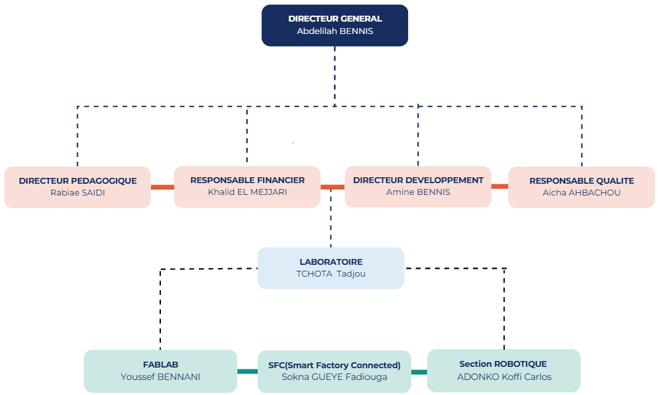
\includegraphics[width=0.9\textwidth]{images/organigramme.png}
	\captionof{figure}{Organigramme de l'HESTIM}
\end{center}

\subsection{Positionnement dans le secteur}

HESTIM s'est imposée comme l'une des écoles d'ingénierie et de management
les plus reconnues au Maroc. Elle bénéficie d'une réputation solide grâce à :

\begin{itemize}
	\item la qualité de ses formations orientées vers les besoins concrets
	du marché ;
	\item ses nombreux partenariats avec des acteurs industriels nationaux
	et internationaux ;
	\item son engagement dans l'innovation pédagogique et technologique,
	notamment dans les domaines de la robotique et de l'intelligence
	artificielle.
\end{itemize}

HESTIM accueille un public varié, marocain et étranger, et cible des
secteurs clés comme l'industrie, les technologies de l'information, le BTP
et la logistique.

\subsection{Valeurs et engagements}

HESTIM place l'innovation, la qualité pédagogique et l'ouverture
internationale au cœur de sa stratégie. L'école vise à former des
ingénieurs et managers capables de répondre aux défis actuels et futurs de
l'industrie, avec un fort accent sur l'éthique, l'esprit d'équipe et
l'adaptabilité aux évolutions technologiques.

\subsection{Lien avec notre stage}

Le stage s'est déroulé au sein de HESTIM, considérée comme l'établissement
d'accueil, car l'école offre un cadre idéal pour mettre en pratique les
connaissances en génie informatique et en intelligence artificielle. La
présence sur site du robot de service Android \textit{CIOT TY1251D-03195} a
permis d'expérimenter directement sur le matériel cible.

Le présent rapport documente la plateforme CYBEL, développée par
Claudia Lusamote Kimfuta ; Ghassane Khalifi a mené en parallèle un travail
complémentaire sur un module chatbot (branche dédiée du dépôt GitHub), non
détaillé dans les chapitres techniques suivants. Grâce aux équipements du
FabLab et à l'environnement de travail du laboratoire, ce stage a permis de
mobiliser des compétences en rétro-ingénierie de protocoles, en
développement d'API et en interfaces homme-robot, en adéquation avec le
programme de la filière Génie Informatique.

\subsection{Conclusion}

La présentation de l'HESTIM Engineering School met en évidence un
environnement académique et technologique favorable à la réalisation de
projets innovants. Sa structure, ses équipements et en particulier la
disponibilité du robot \textit{CIOT TY1251D-03195} et ses formations orientées vers
l'industrie~4.0 ont permis de mener ce stage dans des
conditions optimales, alliant rigueur académique et mise en situation
professionnelle réelle.
